\documentclass[tikz, dvipdfmx]{standalone}
\usepackage{tikz}
\usepackage{tikz-feynhand}
\usetikzlibrary{intersections,calc,arrows.meta}
\begin{document}
  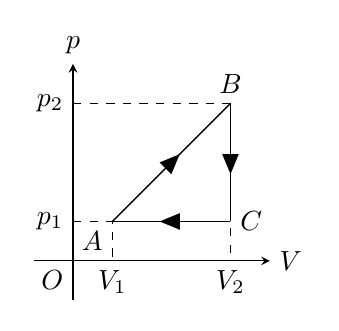
\begin{tikzpicture}
    \coordinate[label=below left:$O$] (O) at (0,0);
    \coordinate (XS) at (-0.5,0);
    \coordinate (XL) at (2.5,0);
    \coordinate (YS) at (0,-0.5);
    \coordinate (YL) at (0,2.5);
    \coordinate[label=below left:$A$] (A) at (0.5,0.5);
    \coordinate[label=above:$B$] (B) at (2,2);
    \coordinate[label=right:$C$] (C) at (2,0.5);
    \coordinate[label=left:$p_1$] (P1) at($(YS)!(A)!(YL)$);
    \coordinate[label=left:$p_2$] (P2) at($(YS)!(B)!(YL)$);
    \coordinate[label=below:$V_1$] (V1) at($(XS)!(A)!(XL)$);
    \coordinate[label=below:$V_2$] (V2) at($(XS)!(B)!(XL)$);
    \draw [->, >=stealth] (XS) -- (XL) node[right]{$V$};
    \draw [->, >=stealth] (YS) -- (YL) node[above]{$p$};
    \draw[dashed] (P1) -- (A) -- (V1);
    \draw[dashed] (P2) -- (B) -- (V2);
    \begin{feynhand}
    \propag[fer] (A) to (B);
    \propag[fer] (B) to (C);
    \propag[fer] (C) to (A);
    \end{feynhand}
  \end{tikzpicture}
\end{document}
